\documentclass[ppsletter,fontsize=11pt,foldmarks=false ]{scrlttr2}
\usepackage[margin=10pt,font=small,labelfont=bf]{caption}
\usepackage{float}
\usepackage{hyperref}
\usepackage{esr}
\usepackage{datatool}

\makeatletter
\@setplength{toaddrvpos}{4.5cm}
\@setplength{toaddrhpos}{12cm}
\KOMAoptions{foldmarks=off}

\DTLsetseparator{;}
\DTLloaddb[noheader,keys={id,sn,gn,mail,c,st,plz,loc,sal,sec,amsec,amsum,num,ref,pref,fdate,fyear}]{people}{people.csv}

% VARIABLES START
\newcommand{\amountpps}{80.00}
\newcommand{\memberid}{13}
\esrEinzahlungFuer{Postfinance\\3030 Bern}
\esrZugunstenVon{Piratenpartei Schweiz\\3000 Bern}
\esrKonto{01-84038-2}
% VARIABLES END

%\setkomavar{memberid}{}
%\setkomavar{membernick}{}
%\setkomavar{memberemail}{}

\setkomavar{partei}{Stefan Thöni}
\setkomavar{departement}{Co-Präsident}
\setkomavar{fromname}{}
\setkomavar{fromstreet}{Piratenpartei Schweiz}
\setkomavar{fromcity}{3000 Bern}
\setkomavar{fromemail}{finance@piratenpartei.ch}
\setkomavar{fromurl}{www.piratenpartei.ch}
\setkomavar{backaddress}{}


\newcommand{\currency}{1}

\begin{document}

\DTLforeach{people}{\id=id,\surname=sn,\givenname=gn,\country=c,\street=st,\postalcode=plz,\location=loc,\salut=sal,\sectionname=sec,\amountsection=amsec,\amountsum=amsum,\invoicenr=num,\reference=ref,\prefix=pref,\facdate=fdate,\facyear=fyear}{%

\setkomavar{date}{\facdate}
\setkomavar{subject}{Rechnung {\invoicenr}}

\selectlanguage{ngerman}

\ifstr{\country}{Switzerland}{%
    \AddToShipoutPicture{\put(0,0){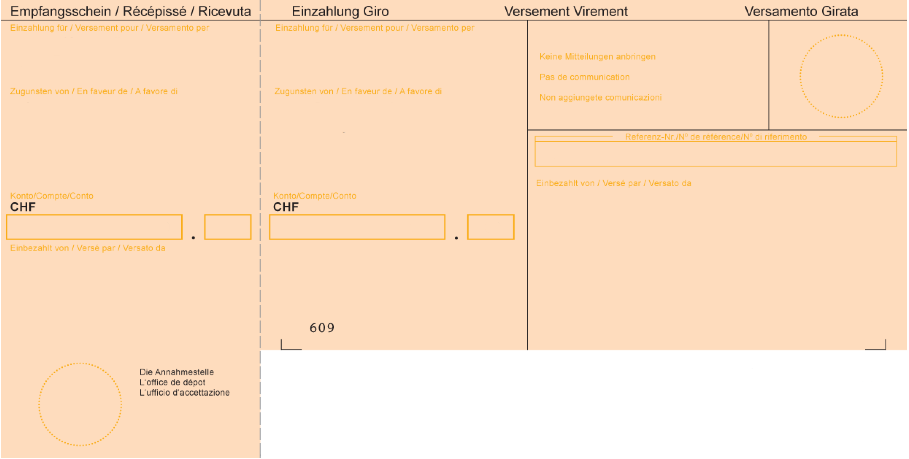
\includegraphics[width=\paperwidth]{orange-pay.png}}
    }
    
    \renewcommand{\currency}{CHF}
}{%
    \renewcommand{\currency}{EUR}
}

\ifstr{\country}{Switzerland}{%

\begin{letter}{%
	\givenname~\surname\\
	\street~\\
	\postalcode~\location\\
	~
}

}{%

\begin{letter}{%
	\givenname~\surname\\
	\street~\\
	\postalcode~\location\\
	\country~
}

}

\enlargethispage{10cm}

\opening{\salut}

Der Mitgliederbetrag setzt sich dieses Jahr wie folgt zusammen:

\ifstr{\sectionname}{\empty}{%

\begin{tabular}{ l l r }
\hspace{8cm}                        &               &                       \\
\textbf{Mitgliedschaft \facyear}    &               & \textbf{Betrag}       \\
Piratenpartei Schweiz               & \currency     & \amountpps            \\
\hline
Total                               & \currency     & \amountsum            \\
\end{tabular}

\vspace{0.5cm}
Die Piratenpartei Schweiz dankt Dir für deine Unterstützung!

}{%

\begin{tabular}{ l l r }
\hspace{8cm}                        &               &                       \\
\textbf{Mitgliedschaft \facyear}    &               & \textbf{Betrag}       \\
Piratenpartei Schweiz               & \currency     & \amountpps            \\
\sectionname                        & \currency     & \amountsection        \\
\hline
Total                               & \currency     & \amountsum            \\
\end{tabular}

\vspace{0.5cm}
Deine Sektion und die Piratenpartei Schweiz danken Dir für deine Unterstützung!

}

\ifstr{\country}{Switzerland}{%

\esrEinbezahltVon{\givenname~\surname \\ \street~ \\ \postalcode~\location}
\expandafter\esrBetrag\expandafter{\amountsum}
\expandafter\esrPrefix\expandafter{\prefix}
\expandafter\esrReferenznummer\expandafter{\reference}
\esrPrint

}{%

\vspace{1cm}
Betrag überweisen an:

Piratenpartei Schweiz \\
3000 Bern

IBAN: CH32 0900 0000 6030 7660 3 \\
BIC: POFICHBEXXX \\
Vermerk: P{\invoicenr}
}

\end{letter}%

}%

\end{document}
